The velocity of wind and  boat are respectively, 
\begin{align}
\vec{v_w} &= 72\myvec{\cos45\degree\\ \sin45\degree} \\
\vec{v_b} &= \myvec{0\\51}
\end{align} 
The resulting wind velocity is
\begin{align}
\vec{v_w}-\vec{v_b} 
&= \myvec{36\sqrt{2}\\36\sqrt{2}-51}
\end{align}
The direction of the flag is 
\begin{align}
\tan^{-1}\brak{\frac{36\sqrt{2}-51}{36\sqrt{2}}}\\
&= -0.1\degree
\end{align}

 The python code for Fig. \ref{fig:3.7.7}
is 
\begin{lstlisting}
solutions/7/codes/line/motion/motion.py
\end{lstlisting}
\begin{figure}[!ht]
\centering
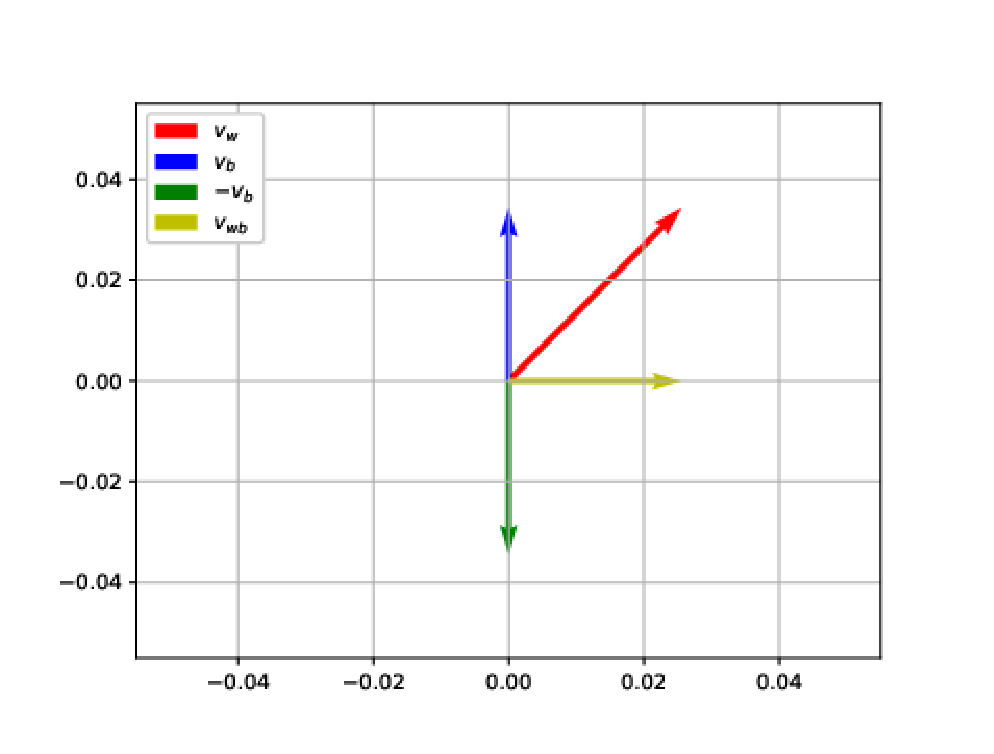
\includegraphics[width= \columnwidth]{./solutions/7/figs/line/motion/motion.eps}
\caption{}
\label{fig:3.7.7}
\end{figure}

